\section{Ziel}
Ziel des Experiments ist, das magnetische Moment freier Elektronen zu messen.

\section{Theorie}
Die Hüllenelektronen eines Atoms, die einen Bahndrehimpuls besitzen, erzeugen ein magnetisches Moment.
Freie Elektronen erzeugen auch ein magnetisches Moment, was auf ihren Eigendrehimpuls zurückzuführen ist.
Der Eigendrehimpuls wird als Spin bezeichnet.
Der Zusammenhang zwischen dem Bahndrehimpuls und magnetischem Moment ist gegeben durch
\begin{equation}
  \mu_z = -\frac{e_0}{2m_0}m\hbar := \mu_Bm,
\end{equation}
wobei $\mu_B$ das Bohrsche Magneton bezeichnet.

Die Wellenfunktion für ein Atom mit einem Außenelektron kann in einen Radialteil und Winkelteil aufgeteilt werden und lautet
\begin{equation*}
  \Psi_{n,l,m}(r,\theta,\phi) = R_{n,l}(r)\Theta_{l,m}(\theta)\Phi(\phi) = R_{n,l}\Theta_{l,m}\frac{\exp(im\phi)}{\sqrt{2\pi}}.
\end{equation*}
Hierbei ist $n$ die Hauptquantenzahl, $l$ die Bahndrehimpulsquantenzahl und $m$ die Orientierungsquantenzahl.
Ein magnetisches Moment, das in ein äußeres homogenes Magnetfeld gebracht wird, enthält die potentielle Energie
\begin{equation*}
  E_{\text{mag}}(m_l) = \mu_z\cdot{B} = m_l\cdot\mu_B\cdot{B}.
\end{equation*}
In einem Magnetfeld kommt es zu einer Aufspaltung der Energieniveaus.
Dies wird als Zeeman-Effekt bezeichnet.
Der Drehimpulsbetrag und die Richtung sind dabei gequantelt.
Die $z$-Komponente (in Magnetfeldrichtung) des Drehimpulses kann die Werte
\begin{align*}
  l_z = m_l \hbar
\end{align*}
annehmen, wobei die Orientierung die Werte
\begin{align*}
  m_l = -l, (-l+1),(-l+2),...,(l-1),l
\end{align*}
also $2l+1$ Einstellmöglichkeiten annehmen kann.
Für den Spin eines Elektrons mit Spinquantenzahl $s = \sfrac{1}{2}$ und Spin-Orientierungsquantenzahl $m_s = \pm\sfrac{1}{2}$ gibt es zwei Einstellmöglichkeiten:
\begin{equation*}
  S_z = m_s\hbar = \pm\frac{1}{2}\hbar.
\end{equation*}
Das zum Spin des Elektrons gehörende magnetische Moment lautet
\begin{equation}
  \mu_{S_z} = -gm_s\mu_B.
\end{equation}
Der Zahlenfaktor $g$ bezeichnet das gyromagnetische Verhältnis bzw. den Landé-Faktor.
Dieses lässt sich mittels Elektronenspin-Resonanz-Methode (ESR) messen.

\section{Prinzip der ESR}
Eine Substanz, die freie Elektronen enthält, wird in ein homogenes Magnetfeld gebracht.
Dadurch kommt es, wie im vorherigen Abschnitt bereits erwähnt zu einer Aufspaltung des Energieniveaus $E_0$ in zwei Energieunterniveaus
\begin{gather*}
  E_0 + \frac{1}{2}g\mu_{B}B, \text{für}\, m_s= +\frac{1}{2},\\
  E_0 - \frac{1}{2}g\mu_{B}B, \text{für}\, m_s= -\frac{1}{2}.
\end{gather*}
Der Energieunterschied der Unterniveaus ist gegeben durch
\begin{equation}
  \Delta E = g\mu_{B}B
\end{equation}
Gemäß der Maxwell-Boltzmann-Statistik ist bei großen Zahlen von Elektronen im thermischen Gleichgewicht der obere Zustand stärker besetzt als der untere.
Das Besetzungsverhältnis ist gegeben durch
\begin{equation*}
  \frac{N(m_s = -\sfrac{1}{2})}{N(m_s = +\sfrac{1}{2})} = \exp\left( \frac{-g\mu_{B}B}{kT} \right)
\end{equation*}
Wird dem System Energie in Form von hochfrequenten (MHz) elektromagnetischen Quanten hinzugeführt, deren Energie gleich der Energiedifferenz der Unterniveaus ist, also
\begin{equation}
  h\nu = g\mu_{B}B,
  \label{eqn:hv}
\end{equation}
dann sind Elektronen in der Lage in den höheren Zustand zu überzugehen.
Der Vorgang dieses "Umklappens" wird Elektronenspin-Resonanz genannt.

Der prinzipielle Aufbau einer Elektronenspinresonanz-Apparatur kann der Abbildung \ref{fig:ESR} entnommen werden.

\begin{figure}[H]
  \centering
  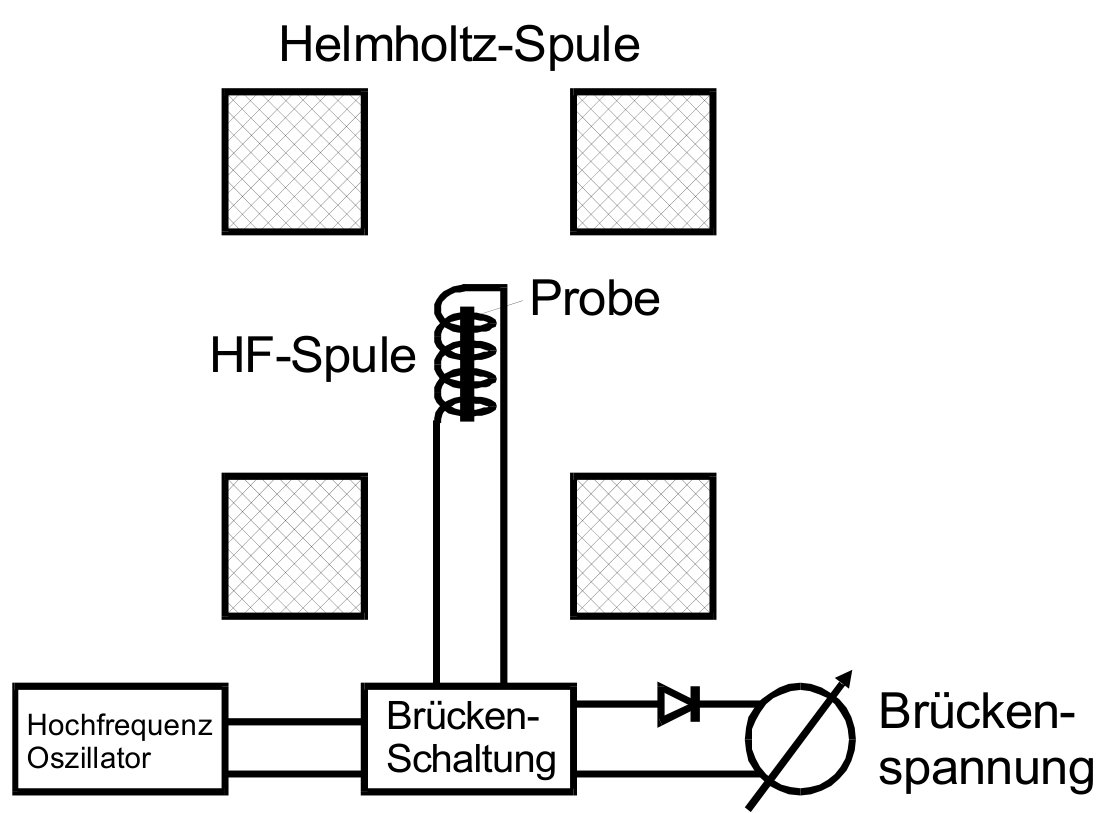
\includegraphics[width=10cm]{ESR.png}
  \caption{Prinzipieller Versuchsaufbau zur Elektronen-Resonanz \cite{skript}.}
  \label{fig:ESR}
\end{figure}

Eine Helmholzspule erzeugt ein homogenes Magnetfeld in dem sich die zu untersuchende Probe befindet.
Das Feld einer Helmholtzspule lässt sich gemäß
\begin{equation}
  B(I) = \frac{8}{\sqrt{125}}\mu_0\frac{n}{r}I
  \label{eqn:B}
\end{equation}
berechnen.
Dabei ist $\mu_0$ die Induktionskonstante, $n$ die Windungszahl der Spule und $r$ der Spulenradius.
Über eine Brückenschaltung, die abgeglichen wird, wird von einem HF-Generator eine weitere Spule gespeist, die um die Probe herumgewickelt ist.
Diese HF-Spule induziert die Elektronenspinresonanz.
Dadurch entsteht außerdem eine Änderung der Magnetisierung der Probe, was wiederum eine Änderung des komplexen Widerstands der HF-Spule bewirkt.
Daraus folgt eine Verstimmung der zuvor abgeglichenen Brücke.
Die entstehende Brückenspannung kann mit einem empfindlichen Voltmeter gemessen werden.
